\documentclass{book}
\usepackage[utf8]{inputenc}
\usepackage[spanish]{babel}
\usepackage{graphicx}
\usepackage{graphicx,subfig}
\usepackage{mathptmx}
\usepackage{multicol}
\usepackage{color}
\usepackage{listings}
\usepackage[usenames,dvipsnames,svgnames,table]{xcolor}

\begin{document}
	\thispagestyle{empty}
	\frontmatter
	
	\section*{TÍTULO}
	\Large{Diseño e implementación de un entorno computacional para la ayuda en la síntesis de sonidos musicales}
	\section*{RESUMEN}
	Con el fin de facilitar la producción de audio con enfoques al público general, de maneja semejante al impacto de herramientas computacionales, se postula la creación de modelos reproducibles y económicos en procesamiento como almacenamiento en memoria sobre un nuevo formato para el desarrollo, en un ambiente computacional integral sencillo de entender y manejar. De esta manera, se espera ofrecer una nueva alternativa a la composición musical que exija menos recursos externos y computaciones en sus formas de almacenar y replicar.
	\section*{OBJETIVOS}
	\begin{itemize}
		\item Construcción de una interfaz de usuario para la ayuda visual y auditiva en la composición y síntesis de sonidos.
		\item Implementación del los modelos generados en otros ambientes de software.
	\end{itemize}
	
	\pagebreak\section*{DEFINICIÓN DEL PROBLEMA}
	La interpretación de información en nuestros medios digitales, nos ha permitido producir y almacenar de forma eficiente y a un nivel mínimo de personal, siendo un ejemplo, solo se requiere un procesador de texto instalado en un equipo para poder construir artículos, publicaciones y gran diversidad de documentos formales, informales, con propósitos de divulgación científica ó de entretenimiento.\par
	Todo lo anterior mencionado, gracias a los productos de software comercial disponibles, tanto en la producción de su contenido objetivo, como sus respectivos entornos de trabajo integrales para su construcción en un proceso más individual ó en un ámbito industrial, como su manutención.\par
	Enlazando ambos conceptos, propongo aplicarlos a un ámbito artístico muy computable gracias a su amplio análisis matemático-lógico. Hablo de la música, disciplina artística de la armonía del sonido, su composición e interpretación, creada a partir de la refinación en las ondas sonoras a gusto y agrado del contexto social.\par 
	Perfectamente replanteadas en modelos trigonométricos, así como la captura de su información con el uso de archivos especializados en su fidelidad, compresión y réplica.
	Visto de otra manera, la información contenida en un archivo de audio, da las instrucciones y valores de comportamiento para un dispositivo de salida sonoro.\par 
	\pagebreak Sin importar el origen de esta información, por una captura directa, una copia de otro archivo, mezclado y renderizado por un programa de edición o incluso de la muy improbable casualidad. Solo se requiere de un método adecuado de producción.\par
	Si el desafío reside en la fuente de origen, entonces se propone \emph{La construcción de una interfaz de usuario para la ayuda visual y auditiva en la composición y síntesis de sonidos.}
	De acuerdo con el teorema de Fourier, referente a la descomposición en señales de onda para cualquier señal periódica. Será la fundamental relación de nuestra propuesta. Pues con la ayuda visual y auditiva en comparar por el oído y vista un modelo generado con respecto a una muestra recolectada, la réplica fidedigna a criterio de la escucha del público objetivo de producto final.\par 
	Esta idea tiene su génesis en el proyecto de sintetizador creado por el usuario \emph{Javidx9/OneLoneCoder}, una plantilla hecha en lenguaje C++ que se puede encontrar en el siguiente repositorio: \color{blue}https://github.com/OneLoneCoder/synth.git \color{black}\\En este se expresan mediante objetos virtuales construidos sobre código duro(Hardcode) funciones trigonométricas de oscilador hechas para la réplica de notas musicales y como en variaciones de amplitud y frecuencia pueden emular instrumentos simplificados.\par
	Así se espera, construir una forma de replicar el audio en tiempo de ejecución, pudiendo aplicar un nuevo panorama de beneficios y propuestas de solución a los ámbitos para la producción de contenido, especialmente aquellas interactivas.\par
	\pagebreak
	\section*{MÉTODO}
	La siguiente imagen muestra una representación simplificada sobre la propuesta de solución al completo, donde se tiene planeadas todas sus funcionalidades y operaciones al menos de cara a un lanzamiento hacia el público interesado, más no uno comercial.\par
	
	Cabe aclarar, este proyecto comprende más objetivos y características para resolver las problemáticas anteriormente planteadas. Aunque por los alcances limitados en tiempo, recursos y personal, se ha decidido centrar los esfuerzos en la parte más significativa en la solución de software, siendo el módulo \emph{Tuner}.
	\begin{figure}[h]
		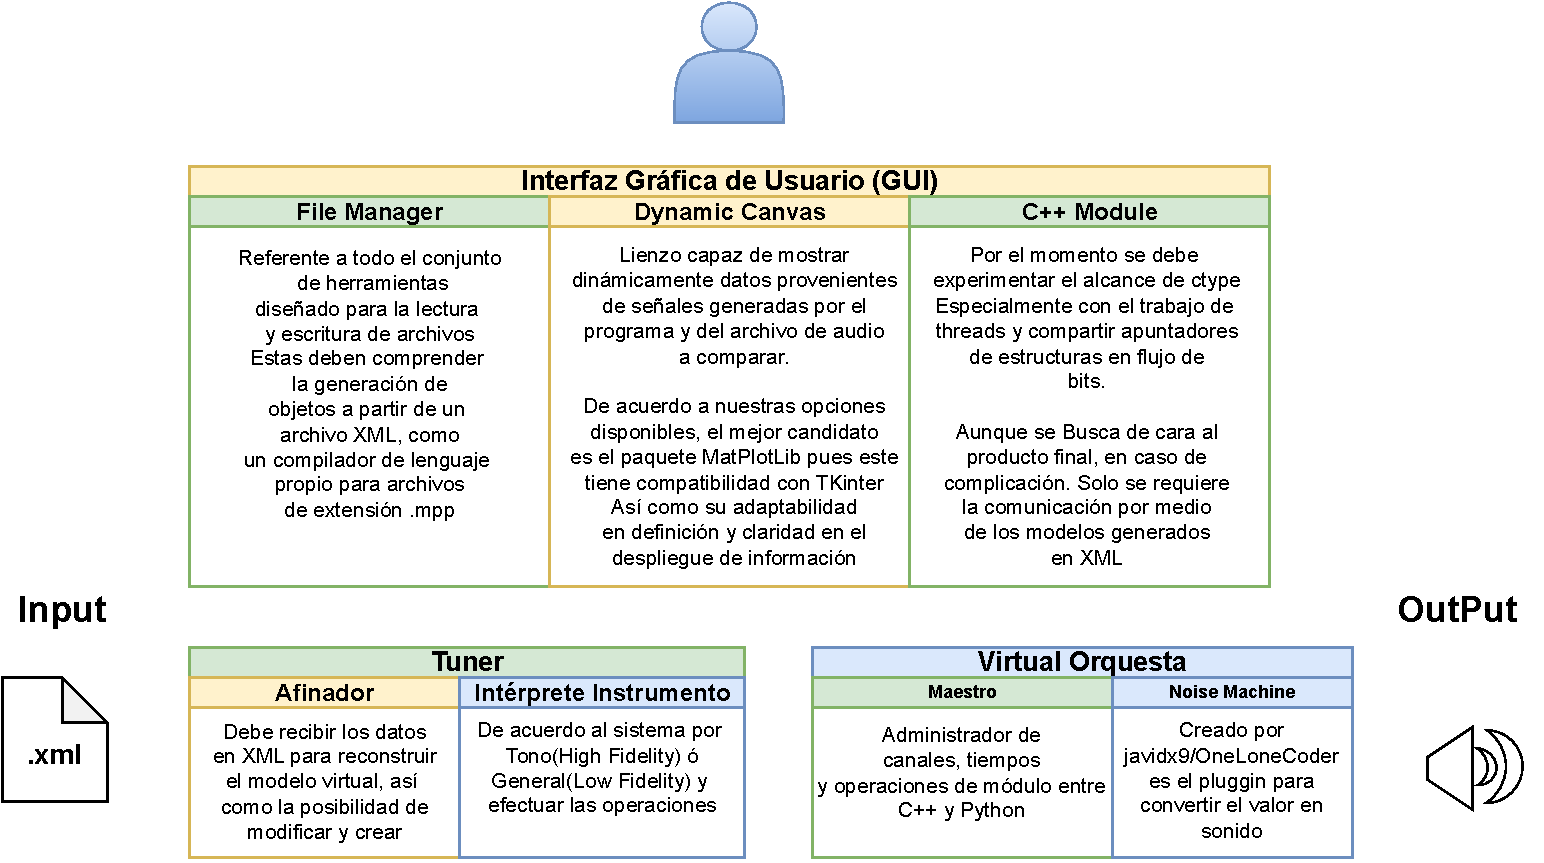
\includegraphics[width=1.25\linewidth]{../Assets/images/musiC++_Diagram_cut}
		\caption{ Diagrama General del Proyecto}
	\end{figure} 
	
	\pagebreak
	Profundizando en los módulos mostrados anteriormente:
	\subsection*{Interfaz Gráfica de Usuario (GUI)}
	El enfoque comercial del proyecto, exige que este contenga por lo menos una visualización cercana a los estándares en herramientas de software, si bien, el público general cambia su tendencia en cuanto conocimientos informáticos básicos, sería un error cerrarnos de cara a una presentación como la manipulación para una terminal de consola. Se ha experimentado construir una GUI con el lenguaje \emph{C++}, sin embargo no pudo encontrarse una biblioteca adecuada, mucho menos un resultado satisfactorio para delegar todo el proyecto a un único lenguaje de programación, por lo tanto, se trabajará con Python en el \emph{FrontEnd}, es decir, todo contacto con el usuario final.\par
	\subsection*{File Manager}
	Ya que nuestro propósito es la generación de archivos cuya información pueda interpretarse por un estándar orientado a audio, así como la preservación del trabajo en un lenguaje de programación, es imperativo usar varios sistemas de lectura y escritura de archivos en ambos lenguajes a utilizar, siendo \emph{Python} y \emph{C++}, estos contienen una biblioteca en sus paquetes fundamentales, siendo la función \emph{open} y \emph{fstream} respectivamente. Por otra parte, se necesitará de una biblioteca especializada en convertir la información de un texto etiquetado como lo es el formato XML. No solo es un estándar que permite escalar las funciones del proyecto a futuro con otros productos de software, sino que al ser un formato simple y en cierto punto, indicativo para ser editado manualmente.
	\subsection*{Dynamic Canvas}
	Si bien, esta parte podría únicamente ser útil en lo que respecta la construcción del módulo afinador. Puede utilizarse en tiempo real la representación gráfica de la información generada, desde los armónicos que participan en la mezcla del sonido, una visión más amigable de cara al usuario de los eventos programados, entre otras cosas. Ya que esto está ligado a la GUI así como el afinador, su desarrollo sería exclusivamente en Python, optando por la opción que ofrece el paquete de \emph{MatPlotLib} por su compatibilidad con \emph{TKinter}.
	\subsection*{C/C++ Module}
	Debido a las características por implementar, es conveniente dejar a Python como aquel que tenga el ejecutable inicial, así como ser el eje de las herramientas que conlleve el proyecto. Este ofrece una opción denominada como \emph{ctype} el cual permite convocar código en \emph{C/C++} colocando y devolviendo datos primitivos, aún no se ha experimentado del todo, pues se requiere de la certeza y técnicas en cuanto el envío de apuntadores para arreglos de datos, estructuras específicas así como su correcto funcionamiento con múltiples hilos de ejecución.
	\pagebreak\subsection*{Tuner}
	Este módulo deberá ser construido en casi su totalidad en lenguaje \emph{Python} pues al comparar en tiempo real la generación de señales, este deberá sumergirse por completo en el ambiente, aunque algunas partes podrían invocarse desde \emph{C/C++} si la eficiencia es significativa. Por otra parte, debe cumplir al menos con la reproducción del modelo concurrente. Así como la lectura de información auditiva escrita en un archivo \emph{.wav} para su comparación ante el modelo generado. 
	\subsection*{Generador de Señales}
	Siendo la parte más visual del proyecto, esta tiene que generar señales con los datos otorgados por el usuario, con representación gráfica en tiempo contra amplitud, frecuencia contra amplitud, frecuencia contra tiempo, en cualquiera pueda ser la información necesaria para la correcta implementación de valores en los modelos matemáticos. Así como la designación de al menos un método de aproximación en comparación a las muestras de audio.
	\subsection*{Virtual Instrument}
	Siendo una convención escrita sobre las reglas del lenguaje de etiquetado XML, es una designación simple y comprensible para la re-construcción de los valores del audio. Consistiendo en 2 secciones, siendo el método, una colección de modelos trigonométricos y una plantilla de señal, siendo una representación de convertir la señal digital absoluta en una transaccional analógica. 
	\pagebreak\subsection*{Virtual Orquesta}
	Este es un módulo enfocado al procesamiento central de la información, pues estará diseñado para invocar la interpretación de las instrucciones y ajustes dados por el usuario, administración de los múltiples hilos dedicados, pausa, reinicio, incluso a la captura en tiempo real de notas generadas por el usuario mediante una entrada estándar así como la posibilidad de escalar a un instrumento especializado.
	\subsection*{MasterChord}
	Siendo esta parte administrativa, deberá cumplir con una facilidad de funciones que puedan ser citadas como servicios desde la GUI así como la respuesta de información siendo instrumentos, posición de notas, tiempo real o cualquier información correspondiente a una visualización con propósitos artísticos o técnicos. Si bien las funciones gráficas son prescindibles, se deja abierta la posibilidad de escalar al producto final.
	\subsection*{NoiseMachine}
	Esta es una cabecera hecha por \emph{Javidx9/OneLoneCoder} que nos permite la comunicación con el hardware hecho para la reproducción de audio mediante la solicitud del tiempo en valor de la amplitud otorgado por una función asignada. Esta pieza limita el proyecto a plataformas con sistema operativo Windows 7 en adelante, con compatibilidad para arquitectura de x32 bits.
	\section*{INVENTARIO DE ASIGNATURAS INVOLUCRADAS}
	Correspondientes al plan de estudios de Ingeniería en Computación(2016)
	\begin{itemize}
		\item Álgebra/Álgebra Lineal
		\item Fundamentos de Física/Programación
		\item Estructuras de datos y algoritmos I/II/Discretas
		\item Cálculo y Geometría Analítica/Integral
		\item Ecuaciones Diferenciales/ Matemáticas Avanzadas
		\item Señales y Sistemas/ Sistemas de Comunicaciones
	\end{itemize}
	\pagebreak\section*{ÍNDICE DESGLOSADO}
	\renewcommand{\theenumii}{\arabic{enumii}}
	\begin{enumerate}
		\item Introducción
		\begin{enumerate}
			\item Objetivo
			\item Planteamiento del problema
			\item Estado del Arte
			\item Fundamentos de la organización Musical
		\end{enumerate}
		\item Análisis y Procesamiento de Audio
		\begin{enumerate}
			\item Definición Técnica del Audio
			\item Captura de Información
			\item Procesamiento de Señal
			\item Métodos de aproximación
		\end{enumerate}
		\item Construcción de la NoiseMachine
		\begin{enumerate}
			\item Estudio del proyecto olcSynth
			\item Aporte de propuesta
			\item Cambios y pruebas del software
			\item Implementación y Proyección a Futuro
		\end{enumerate}
		\item Construcción del Tunner
		\begin{enumerate}
			\item Estrategia y Diseño
			\item Manejo de excepciones
			\item Capacidades mínimas
			\item Áreas de Innovación
		\end{enumerate}
		\pagebreak\item Diseño de los Instrumentos Virtuales
		\begin{enumerate}
			\item Resumen de XML
			\item Propuesta de Convención
			\item Proyecciones con musiC++
			\item Comparación contra formatos estandarizados
		\end{enumerate}
		\item Guía de Usuario
		\begin{enumerate}
			\item Paso 1: Recolección de Muestra
			\item Paso 2: Afinar el Instrumento Virtual
			\item Paso 3: Prueba de Sonido
			\item Paso 4: Exportación a otros Productos
		\end{enumerate}
		\item Conclusiones
		\item Bibliografía
		\item Anexos
	\end{enumerate}\pagebreak
	\section*{RESULTADOS ESPERADOS}
	Con el entorno de producción finalizado, se espera obtener en referencia al producto, como en propuesta de uso:
	\begin{itemize}
		\item Nuevo Formato de Almacenamiento de información orientado al arte musical
		\item Modelos Instrumentales digitales utilizables en otros proyectos de programación
		\item Facilidad en su comprensión para el usuario en su fabricación de Instrumentos virtuales
		\item Simulación de instrumental precisa y universal
		\item Diseño escalable al número de funciones y modos de interpretación del sonido producido
		\item Independencia de periféricos instrumentales reales
	\end{itemize}
	Cuando se ha mencionado el proyecto del génesis, podemos observar un área de oportunidad mucho más grande, pues si retornamos y vemos la versión \emph{main4.cpp} integra la clase secuenciador, una muy simplificada automatización en añadir notas al proceso. Esto puede significar que una completa melodía podría implementarse de forma concreta bajo este sistema, adicionalmente a este proyecto, se podían componer canciones o replicar las existentes con los instrumentos virtuales de este proyecto, en este conjunto de soluciones propuestas.\pagebreak\par
	
	Citando un ejemplo más específico, en la industria del entretenimiento digital como lo son los videojuegos, entornos virtuales variables sujetos a la interacción usuario computadora, donde gracias a esta propuesta se podría brindar una experiencia sonora artística mucho más apta y factible. Un alto punto de valor agregado que puede significar muchas más ganancias, prestigio y un nuevo paradigma.\par
	
	\section*{CRONOGRAMA}
	\begin{figure}[h]
		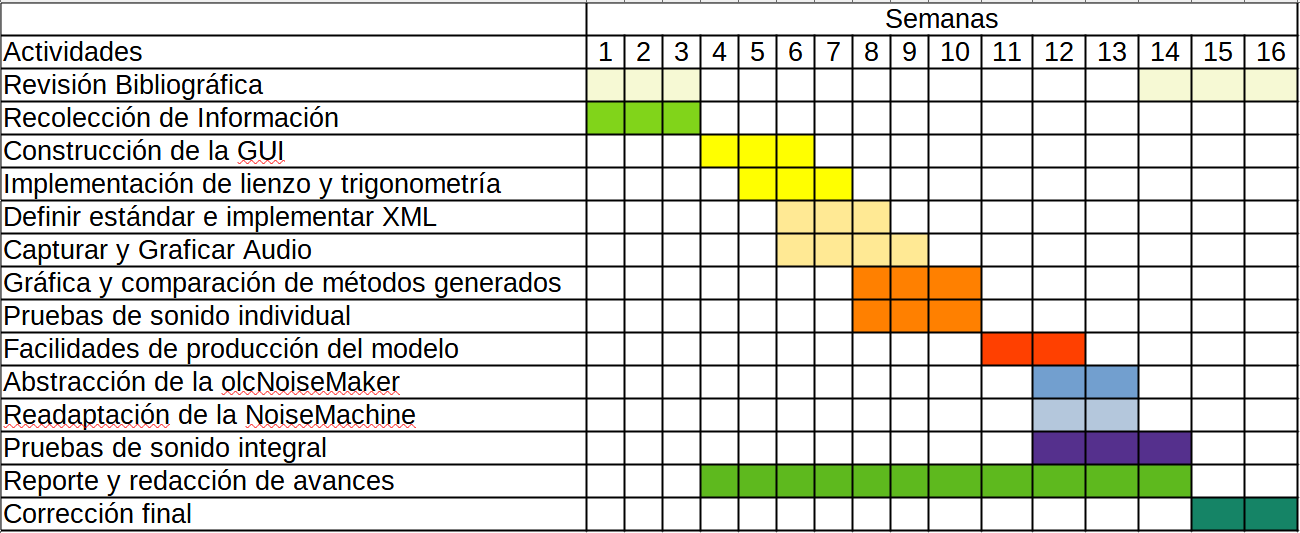
\includegraphics[width=\linewidth]{../Assets/images/cronograma}
		\caption{Planeación estimada del desarrollo}
	\end{figure} 
\end{document}

